\documentclass[conference]{IEEEtran}
\IEEEoverridecommandlockouts
\usepackage{amsmath,amssymb,amsthm}
\usepackage{fontspec}
\setmainfont{texgyretermes}[Extension=.otf, UprightFont=*-regular, BoldFont=*-bold, ItalicFont=*-italic, BoldItalicFont=*-bolditalic]
\usepackage{unicode-math}
\setmathfont{texgyretermes-math.otf}
\usepackage{graphicx}
\usepackage{booktabs}
\usepackage{multirow}
\usepackage[hidelinks]{hyperref}
\graphicspath{{../results/figures/}}

\newtheorem{proposition}{Proposition}
\theoremstyle{definition}
\newtheorem{definition}{Definition}
\newtheorem{assumption}{Assumption}

\begin{document}

\title{Conformal Calibration of Open-Vocabulary Semantic Maps under Label and Pose Uncertainty%
\thanks{Code and data: \url{https://github.com/byoverr/label-pose-conformal-nav}.}}

\author{\IEEEauthorblockN{Sergey Shchetinkin}
\IEEEauthorblockA{ITMO University, Saint Petersburg, Russia}}

\maketitle

\begin{abstract}
A robot that avoids ``the plant'' on an open-vocabulary semantic map is exposed to two errors at once. The detector
misses, truncates or mislabels objects, and the pose estimate drifts, so objects are drawn in the wrong place.
Existing distribution-free guarantees for planning on perception maps calibrate the first error and assume a known
pose. We calibrate one per-scene quantity, the \emph{miss distance}: the directed Hausdorff distance from the true
footprints of a class to the class region on the map built with estimated poses, measured in the planner's frame.
Its split-conformal quantile is a keep-out margin. Any path that stays this margin plus the safety distance away from
the class region is safe with the target probability, whichever planner produced it. On 21 OSMa-Bench scenes the
joint margin keeps $0.93$ coverage at a $0.9$ target from zero to 45~cm of drift, while margins calibrated on labels
or on pose alone lose coverage. In the setting of the closest prior work, known pose and a closed vocabulary,
label-set calibration and ours achieve the same mission success. With drift or an open vocabulary ours keeps its
guarantee and succeeds more often. With real visual odometry and no loop closure the method abstains instead of
issuing a false certificate.
\end{abstract}

\section{Introduction}

Open-vocabulary semantic maps~\cite{conceptgraphs} let a robot follow instructions such as ``keep away from the
bike''. The map has two unreliable inputs. A detector or segmenter supplies the labels, and it misses objects,
covers them only in part, or confuses classes. The robot's pose estimate places the observations, and it drifts.
Planners usually take the map at face value and keep a fixed clearance from the regions of avoid classes.

How unsafe this is usually goes unmeasured. OSMa-Bench~\cite{osmabench} shows that open-vocabulary maps degrade
sharply under lighting changes (the f-mIoU of ConceptGraphs drops from 28.00 to 14.29), but it scores the map as an
image, without a robot moving through it. A recent survey of 3D scene graphs~\cite{survey3dsg} lists the link between
map errors and robot behaviour as an open problem.

Conformal prediction (CP)~\cite{gentle} gives a planner guarantees without assumptions on the error distribution.
Sundarsingh et al.~\cite{sundarsingh} calibrate per-cell label sets of a semantic grid; Perceive With
Confidence~\cite{pwc} calibrates how much to inflate an occupancy map. Both assume that the robot's pose is known,
and separately calibrated modules need not form a calibrated system~\cite{baral}.

We ask what guarantee a planner gets when label error and pose error act together, and how to calibrate it. Our
contributions are:
\begin{itemize}
  \item a nonconformity score, the miss distance, measured in the planner frame on a map built with estimated poses;
  its per-class conformal quantile is a margin that covers both errors for any planner;
  \item an evaluation on 21 OSMa-Bench scenes with six levels of synthetic drift and real visual odometry, which
  shows that margins calibrated on one error lose coverage under the other and that the sum of two separate margins
  either over-pays or under-covers, depending on how the errors are distributed over scenes;
  \item a comparison with label-set calibration~\cite{sundarsingh} in its own setting and in ours, which explains why
  label-space calibration degenerates on indoor maps.
\end{itemize}

\section{Related Work}

\textbf{Open-vocabulary mapping.} ConceptGraphs~\cite{conceptgraphs} fuses class-agnostic masks into an object graph
with CLIP features; OSMa-Bench~\cite{osmabench} and OSMa-Bench++~\cite{osmabenchpp} evaluate such mappers under
lighting changes. Naive Bayesian fusion makes semantic maps over-confident~\cite{overconf}; we fuse by averaging.
None of these works evaluates the map through a motion task.

\textbf{Conformal guarantees for planning.} CP entered planning through trajectory prediction of other
agents~\cite{lindemann}. Shin et al.~\cite{shin2026} conformalize the whole distance field to moving obstacles and
obtain a constraint that certifies any MPC trajectory; semantics and the robot's own pose error are outside their
scope. Learnable CP~\cite{learnablecp} learns a context-aware score for RRT$^\ast$ clearance, and constraint
tightening~\cite{tightening} shows that tightened constraints are safe for any planner. Closest to us, Sundarsingh et
al.~\cite{sundarsingh} calibrate label sets of grid cells with one score per environment (the worst cell) and plan
with the most conservative label of each cell. They report 93.4\,\% correct maps and 98.4\,\% mission success at a
95\,\% target, with a known pose, five classes and a 1~m grid on $70\times25$~m outdoor sites. Perceive With
Confidence~\cite{pwc} calibrates the smallest inflation of an occupancy map that covers all obstacles; our score is a
semantic counterpart of theirs that also absorbs pose error.

\textbf{Composition and pose error.} Two modules calibrated at 95\,\% give between 86 and 99.98\,\% after
composition depending on error correlation, and joint calibration restores the target~\cite{baral}.
Calafiore~\cite{calafiore2026} combines blockwise certificates through a union bound with an explicit risk budget; in
his example a joint calibration of the supremum residual gives a slightly tighter margin. Pose error in semantic
memory is real and poorly calibrated: on a real robot the nominal 95\,\% pose ellipsoid covers a third of the actual
errors~\cite{pposemem}. We found no prior work that calibrates open-vocabulary label error and pose error jointly
with a planner in the loop; the claim rests on a citation and keyword search of October 2026.

\section{Problem Formulation}\label{sec:problem}

A scene $\Omega$ is drawn from an unknown distribution $\mathcal D$. It contains objects of avoid classes
$\mathcal K$; object $e$ has class $k_e$ and floor footprint $F_e \subset \mathbb R^2$, and
$F_k = \bigcup_{e:\,k_e = k} F_e$. The robot moves along true poses $T_1, \dots, T_q \in SE(2)$, and its estimator
returns $\hat T_t = D_t T_t$ with accumulated error $D_t \in SE(2)$, $D_1 = I$. A grid map $\hat M$ is fused from all
observations placed with the \emph{estimated} poses; cell $j$ stores the score-weighted fraction $p_j(k)$ of its
observations that support class $k$. The region of class $k$ at threshold $\lambda$ is
\begin{equation}
  A_\lambda(k) = \{\, j : j \text{ occupied},\ p_j(k) \ge \lambda \,\}.
\end{equation}
The planner acts at time $q$ in the world as the robot believes it to be. An object seen at time $t$ is drawn with
error $D_t$, while the robot sits with error $D_q$, so in the planner frame the true footprint is
$\hat F_k = D_q F_k$. A constant pose error moves the map and the robot together and is harmless; the difference
between the error at observation time and at query time is what hurts.

A path $\gamma\colon[0, 1] \to \mathbb R^2$ is safe for class $k$ if $\operatorname{dist}(\gamma(\tau), \hat F_k) \ge d$
for all $\tau$. Given $n$ calibration scenes with known ground truth, we seek per-class margins $r_k$ that are as small
as possible and satisfy, for a new scene,
\begin{equation}
  \mathbb P\Bigl(\begin{array}{l}\text{every path with } \operatorname{dist}(\gamma, A_\lambda(k)) \ge d + r_k\\ \text{is safe for class } k\end{array}\Bigr) \ge 1 - \alpha.
  \label{eq:goal}
\end{equation}
The probability is over the calibration scenes, the new scene and the error realizations.

\begin{assumption}[exchangeability]\label{as:exch}
The calibration scenes $\Omega_1, \dots, \Omega_n$ and the new scene $\Omega_{n+1}$ are exchangeable.
\end{assumption}

No model of the detector or of the pose estimator is needed. We test four hypotheses: a margin calibrated at the true
pose loses coverage once drift is comparable to the label error (H1); a margin calibrated with ground-truth labels
under-covers while drift is smaller than the label error (H2); the joint margin of Sec.~\ref{sec:method} keeps
coverage at every drift level and is smaller than the sum of the two (H3); map mIoU is a poor predictor of mission
safety (H4).

\section{Method}\label{sec:method}

\begin{definition}[miss distance]
For scene $\Omega$ and class $k$,
\begin{equation}
  s_k(\Omega) = \min\bigl\{R_{\max},\ h\bigl(\hat F_k, A_\lambda(k)\bigr)\bigr\},
  \label{eq:miss}
\end{equation}
where $h(X, Y) = \sup_{x\in X} \inf_{y\in Y} \|x - y\|$ is the directed Hausdorff distance from the true footprints to the class region; $s_k = 0$ if the scene has no object of
class $k$ and $s_k = R_{\max}$ if the region is empty.
\end{definition}

A missed or mislabeled object gives a large score, a truncated object gives the length of the missing part, and a pose
shift gives the size of the shift. Both errors enter one number in the way they affect the planner. We compute one
score per scene: cells, frames and objects of one scene are strongly dependent and are not exchangeable units.

\textbf{Calibration.} Let $s^{(1)} \le \dots \le s^{(n)}$ be the sorted calibration scores of class $k$ and
$m = \lceil (n + 1)(1 - \alpha) \rceil$. The margin is $\hat r_k = s^{(m)}$. If $m > n$ (that is,
$n < 1/\alpha - 1$) or $\hat r_k \ge R_{\max}$, the class \emph{abstains}: its certificate is vacuous. Calibrating per
class keeps one unreliable class from inflating the others.

\begin{proposition}\label{prop:valid}
Under Assumption~\ref{as:exch}, $\mathbb P(s_k(\Omega_{n+1}) \le \hat r_k) \ge 1 - \alpha$, and $r_k = \hat r_k$
satisfies~\eqref{eq:goal}.
\end{proposition}
\begin{proof}
By exchangeability the rank of $s_k(\Omega_{n+1})$ among the $n + 1$ scores is uniform (ties broken in favour of
coverage), so $\mathbb P(s_k(\Omega_{n+1}) \le s^{(m)}) \ge m/(n + 1) \ge 1 - \alpha$~\cite{gentle}. If
$s_k \le \hat r_k$, every $y \in \hat F_k$ has some $a \in A_\lambda(k)$ with $\|y - a\| \le \hat r_k$. For a path point
$x$ with $\operatorname{dist}(x, A_\lambda(k)) \ge d + \hat r_k$, the triangle inequality gives
$\|x - y\| \ge \|x - a\| - \|a - y\| \ge d$.
\end{proof}

The certificate does not depend on the planner; the planner only decides whether a path exists in the narrowed free
space. With $n = 13$ and $\alpha = 0.1$, $m = 13$ and the margin is the largest calibration score.

\textbf{Compared calibrations.} All arms use the same region $A_{\lambda_0}(k)$, with $\lambda_0 = 0.05$ chosen on a
development scene, and differ in the scores the margin is calibrated on: \emph{uncalibrated} (margin 0);
\emph{labels only}, score~\eqref{eq:miss} on the detector map at true poses, giving $r^{\mathrm{lab}}_k$; \emph{pose
only}, the same score on a ground-truth-label map built with drifted poses, giving $r^{\mathrm{pose}}_k$;
\emph{separate}, $r^{\mathrm{lab}}_k + r^{\mathrm{pose}}_k$ with both at level $\alpha$; and \emph{joint}, the score
on the detector map built with drifted poses. We also re-implement \emph{label sets}~\cite{sundarsingh}: the score is
the worst $1 - p_j(k)$ over true footprint cells, the threshold is $\lambda^\ast = 1 - \hat q$ with $\hat q$ its
conformal quantile, and every cell whose label set contains $k$ is avoided.

\begin{proposition}\label{prop:sep}
If $s_k \le s^{\mathrm{lab}}_k + s^{\mathrm{pose}}_k$ for the scores of the same scene, the separate margin has
coverage at least $1 - 2\alpha$, not $1 - \alpha$.
\end{proposition}
\begin{proof}
Each margin fails to cover its own score with probability at most $\alpha$. By the union bound both cover with
probability at least $1 - 2\alpha$, and then $s_k \le r^{\mathrm{lab}}_k + r^{\mathrm{pose}}_k$.
\end{proof}

A risk budget of $\alpha/2$ per module~\cite{calafiore2026} restores $1 - \alpha$ but needs $n \ge 2/\alpha - 1$,
that is 19 calibration scenes at $\alpha = 0.1$. Where the sum lands between $1 - 2\alpha$ and 1 depends on the
dependence of the two errors, which is unknown in practice. The joint margin does not depend on it.

\textbf{Missions.} A robot of radius 0.2~m must reach a goal. The keep-out zone of class $k$ is
$A_{\lambda_0}(k)$ dilated by $d + r_k$, with $d = 0.5$~m. Dijkstra's algorithm on the 8-connected grid finds the
shortest path; it is complete, so ``no path'' means that none exists. A path is \emph{unsafe} if it comes closer than
$d$ to a true avoid object in the planner frame; a mission \emph{succeeds} if a safe path is found. The same planner
on the true map serves as an oracle.

\section{Experimental Setup}

\textbf{Data and perception.} We use 22 ReplicaCAD scenes of OSMa-Bench~\cite{osmabench,habitat2} with RGB-D,
ground-truth semantics and poses at $640\times480$, every 8th frame. All design choices were made on
\texttt{apt\_0}; the other 21 scenes are split 200 times at random into 13 calibration and 8 test scenes.
YOLO-World v2-s~\cite{yoloworld} runs with the 98 object classes of the dataset as prompts; inside each box we keep
pixels within 0.25~m of the median box depth. Maps are 5~cm grids, and points 0.1--1.8~m above the floor are
obstacles. The avoid classes are indoor plant, bike and TV stand.

\textbf{Pose error.} Synthetic drift replays every relative motion of the true trajectory with planar noise
proportional to the distance travelled and the angle turned. Six levels are set once on the development scene by target
absolute trajectory error (ATE). On the evaluation scenes, whose paths are shorter, the median ATE is 0.4~cm (L1),
2~cm (L2), 7~cm (L3), 45~cm (L4, 3.6\,\% of the path) and 2.7~m (L5); we draw 10 realizations per level. As real pose
error we run frame-to-frame RGB-D odometry of Open3D~\cite{open3d,steinbrucker} on every 2nd frame with a planar
ground-robot constraint and no loop closure, without tuning it on ground truth.

\textbf{Protocol and tasks.} $\alpha = 0.1$ unless stated, $R_{\max} = 3$~m; abstention counts as vacuous coverage and
is reported. Start and goal are at least 1.5~m from avoid objects and 3~m apart. \emph{Hard} tasks are selected so that
the shortest obstacle-free path passes within 0.5~m of a plant or bike (233 tasks in 15 scenes); \emph{random} tasks
are not selected (20 per scene). Margins for a scene are calibrated on all other scenes. A class that abstains falls
back to treating every occupied cell as that class.

\section{Results}

\subsection{Coverage under pose drift}

\begin{table}[t]
\centering
\caption{Coverage and median margin (m) for bike and plant, $1 - \alpha = 0.9$. Median ATE: L2 2~cm, L4 45~cm.
$^\dagger$ the arm abstains in at least half of the splits; the margin of the others is shown.}
\label{tab:coverage}
\setlength{\tabcolsep}{3pt}
\footnotesize
\begin{tabular}{l|ccc|c|ccc|c}
\toprule
 & \multicolumn{4}{c|}{bike} & \multicolumn{4}{c}{indoor plant} \\
calibration & L0 & L2 & L4 & $\hat r$ L4 & L0 & L2 & L4 & $\hat r$ L4 \\
\midrule
uncalibrated & 0.00 & 0.00 & 0.01 & 0 & 0.00 & 0.00 & 0.00 & 0 \\
label sets~\cite{sundarsingh} & 1.00 & 0.73 & 0.17 & --- & 1.00 & 0.41 & 0.03 & --- \\
labels only & 0.93 & 0.94 & 0.76 & 0.75 & 0.93 & 0.96 & 0.86 & 0.85$^\dagger$ \\
pose only & 0.00 & 0.03 & 0.82 & 0.90 & 0.00 & 0.00 & 0.86 & 1.39 \\
separate & 0.93 & 0.98 & 0.97 & 1.61 & 0.93 & 0.98 & 0.95 & 2.11$^\dagger$ \\
\textbf{joint (ours)} & \textbf{0.93} & \textbf{0.94} & \textbf{0.93} & \textbf{1.18} & \textbf{0.93} & \textbf{0.93} & \textbf{0.93} & \textbf{1.53}$^\dagger$ \\
\bottomrule
\end{tabular}
\end{table}

Table~\ref{tab:coverage} tests H1--H3. The uncalibrated map almost never contains the whole true footprint, because
the detector truncates object edges. Label sets reach 1.00 at the true pose only through $\lambda^\ast = 0$, which
declares every occupied cell possibly hazardous; with no metric slack, 2~cm of drift drops their coverage to 0.73. The
labels-only margin holds while drift stays below the label error (up to 7~cm) and falls to 0.76 at 45~cm (H1). The
pose-only margin cannot see detector errors and stays at or below 0.22 up to 7~cm (H2). The joint margin holds
0.93--0.94 at every level and at 45~cm is 27--28\,\% smaller than the sum of separate margins (H3).

The plant abstains in about 60\,\% of the splits because the detector misses it completely in one scene, and with 13
calibration scenes the margin is the maximum. The TV stand abstains in 71--95\,\% of the splits: in 2 of 21 scenes the
detector confidently labels it as a bench or a rug. For this detector the TV stand cannot be certified at 90\,\%, and
the calibration says so.

\subsection{Missions}

\begin{figure}[t]
\centering
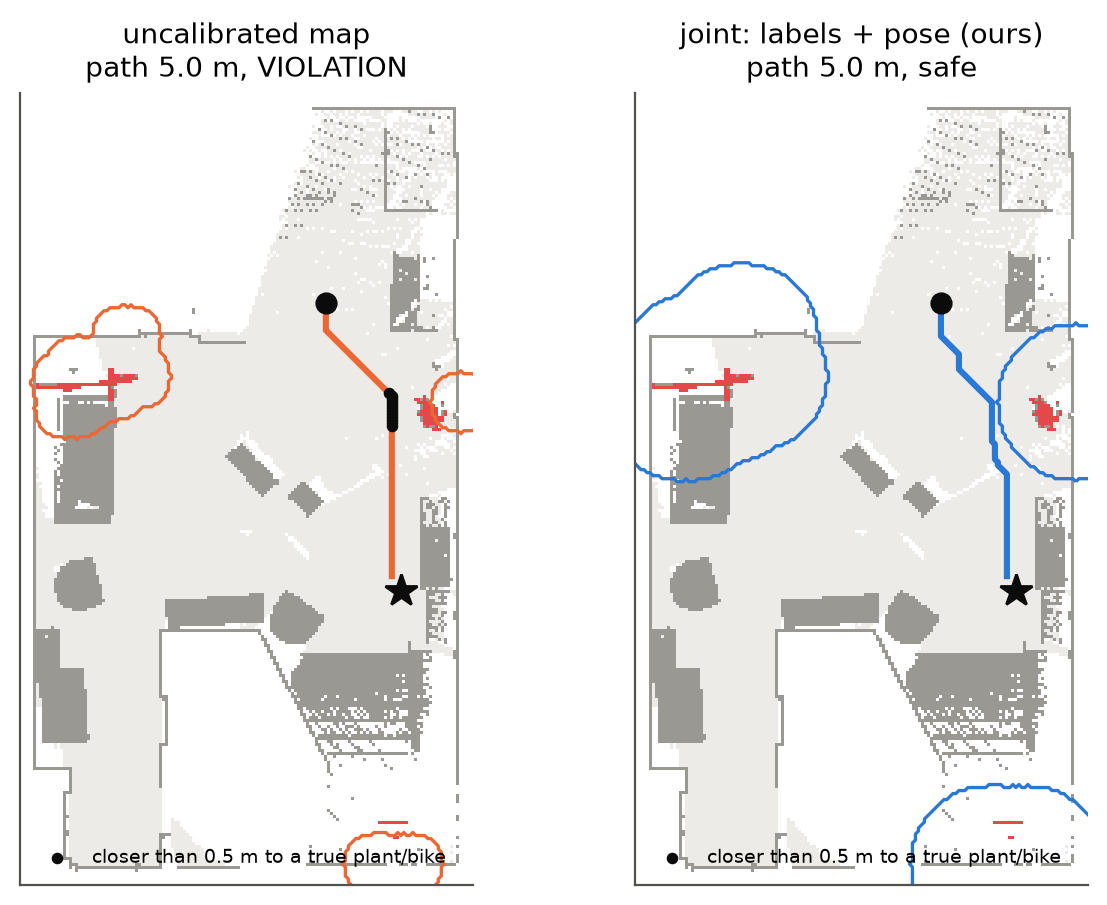
\includegraphics[width=\linewidth]{example_v3_sc0_staging_20_paper.png}
\caption{A hard task at L2. Red: true plant and bike; line: keep-out boundary. The uncalibrated zone misses part of
the plant and the path passes within 0.5~m of it (black dots); the joint zone covers it.}
\label{fig:example}
\end{figure}

On hard tasks the uncalibrated planner almost always finds a path, but 27--37\,\% of its paths are unsafe at L0--L3
(Fig.~\ref{fig:example}). Every calibrated arm has no unsafe path at any level. The price is that a path exists in
only 30--32\,\% of these deliberately hard tasks, against 98--100\,\% on the true map. On random tasks the joint margin
gives 78\,\% successful missions at the true pose and 68\,\% at L3, with no unsafe one; the uncalibrated planner
succeeds in 95 and 82\,\%, but 4--6\,\% of its missions are unsafe. Map quality does not predict safety: across scenes,
the Spearman correlation between mIoU and the violation rate of the uncalibrated planner is $-0.16$ ($p = 0.57$, 15
scenes), which supports H4.

\subsection{Comparison with label sets in their setting}

\begin{table}[t]
\centering
\caption{Random tasks: coverage (minimum over plant and bike), mission success and unsafe missions.}
\label{tab:comparison}
\setlength{\tabcolsep}{3pt}
\footnotesize
\begin{tabular}{ll|ccc|ccc}
\toprule
 & & \multicolumn{3}{c|}{label sets~\cite{sundarsingh}} & \multicolumn{3}{c}{\textbf{joint (ours)}} \\
setting & drift & cov. & succ. & unsafe & cov. & succ. & unsafe \\
\midrule
\multirow{3}{*}{\shortstack[l]{closed vocab.,\\ $1-\alpha = 0.95$}} & none & 1.00 & 0.43 & 0.000 & 0.94 & 0.42 & 0.000 \\
 & 2 cm & 0.42 & 0.40 & 0.000 & 0.94 & 0.61 & 0.000 \\
 & 7 cm & 0.10 & 0.32 & 0.002 & 0.94 & 0.50 & 0.000 \\
\midrule
\multirow{3}{*}{\shortstack[l]{open vocab.,\\ $1-\alpha = 0.9$}} & none & 1.00 & 0.43 & 0.000 & 0.93 & 0.78 & 0.000 \\
 & 2 cm & 0.41 & 0.40 & 0.000 & 0.93 & 0.74 & 0.000 \\
 & 7 cm & 0.10 & 0.32 & 0.002 & 0.94 & 0.68 & 0.000 \\
\bottomrule
\end{tabular}
\end{table}

\begin{figure*}[t]
\centering
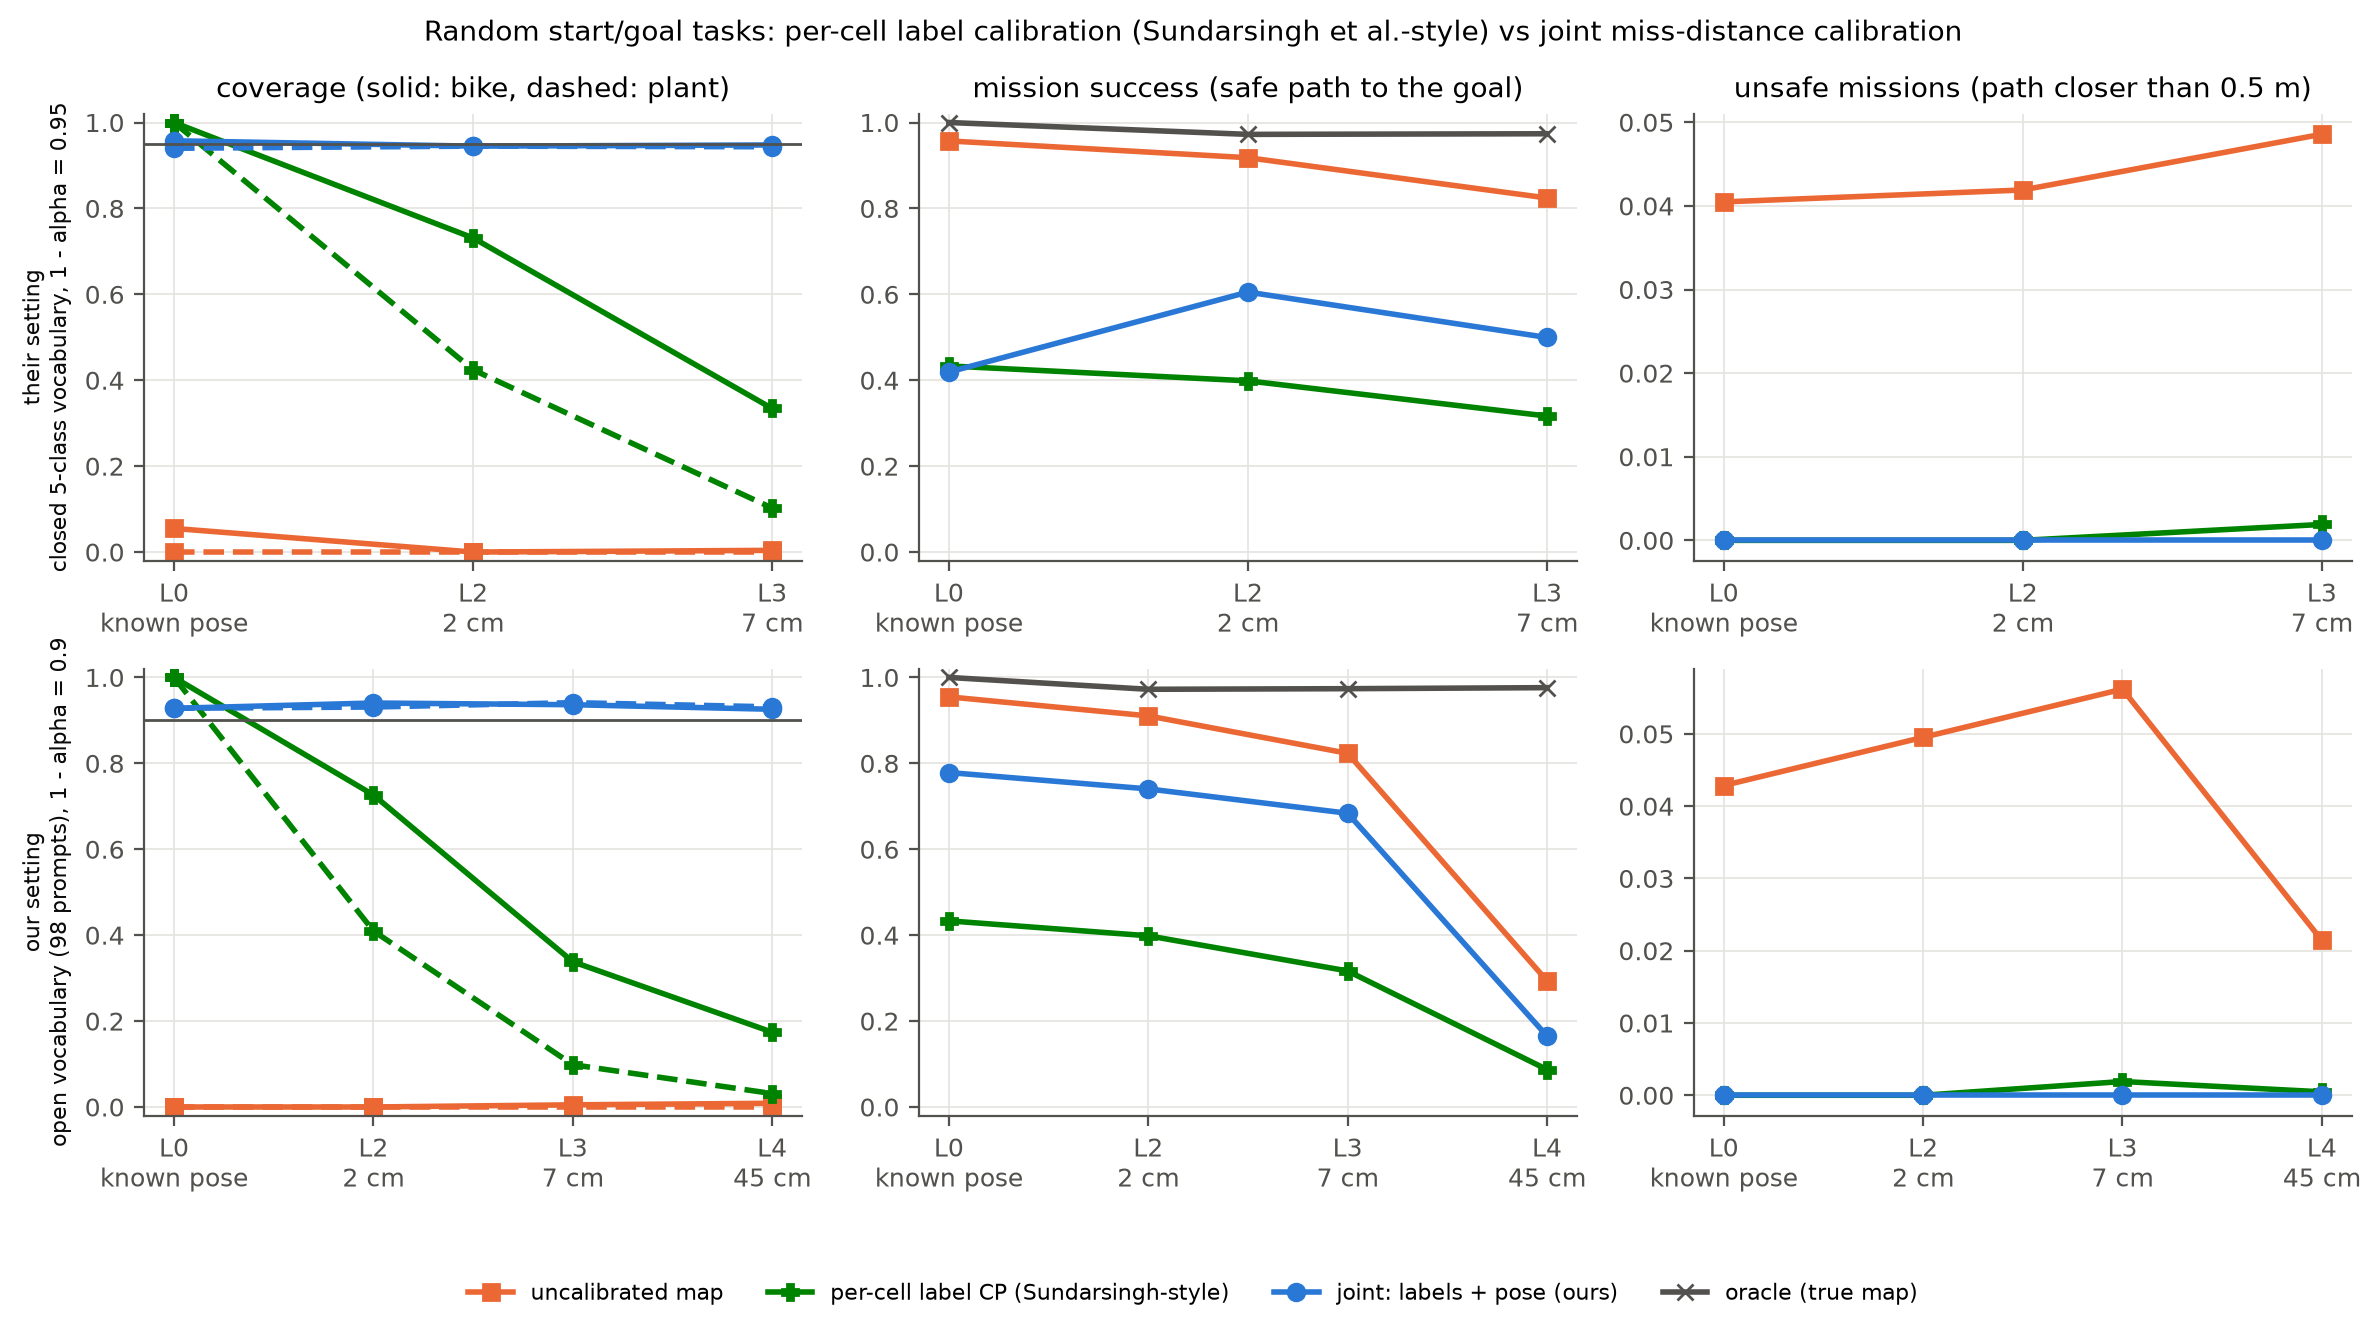
\includegraphics[width=0.88\textwidth]{comparison.png}
\caption{Label sets~\cite{sundarsingh} and the joint margin on random tasks. Top: closed vocabulary, $1-\alpha=0.95$;
bottom: open vocabulary, $1-\alpha=0.9$.}
\label{fig:comparison}
\end{figure*}

The mission success of~\cite{sundarsingh} comes from a different setting, so we compare the methods on our scenes under
their assumptions: known pose, a closed vocabulary of five classes (five rows of the detector's prompt embeddings,
which is equivalent to re-prompting it), $1 - \alpha = 0.95$ and random tasks. Their exploration mode is not
reproduced. In their setting the two calibrations are equal (0.43 vs.\ 0.42 mission success, no unsafe missions;
Table~\ref{tab:comparison}, Fig.~\ref{fig:comparison}). With 2 and 7~cm of drift the coverage of label sets falls to
0.42 and 0.10, while the joint margin stays at 0.94 and succeeds more often (0.61 and 0.50 vs.\ 0.40 and 0.32). With the
open vocabulary the joint margin succeeds 1.8 times as often already at the true pose.

Why do label sets degenerate here? Their threshold is $\lambda^\ast = 0$ with both vocabularies. We suspected the fine
grid and repeated both calibrations at the true pose on grids of 5, 25, 50 and 100~cm. The threshold is zero at every
resolution, and the keep-out zone of label sets takes 64\,\% of the free space at 5~cm and all of it at 1~m. The cause
is complete misses: if in one calibration scene no observation of the class reaches part of the object, the worst cell
scores 1 and the threshold drops to zero. A label set can only say ``this cell may be a plant''. A distance says ``a
plant is nearby'', which stays informative when the detector loses parts of objects.

\subsection{The price of the guarantee}

Raising the risk level barely helps. From $\alpha = 0.1$ to $0.3$ the joint margin shrinks by 0.2--0.25~m and the share
of hard tasks with a path goes from 30 to 31\,\% at L3, while coverage tracks $1 - \alpha$ (0.94, 0.87, 0.72 at
$\alpha = 0.1, 0.2, 0.3$). Better masks do not shrink the margin either. MobileSAM~\cite{mobilesam} prompted with the
detector boxes cuts the median bike miss from 0.43 to 0.05~m, but the worst scene keeps a 0.75~m miss and, with 13
calibration scenes, sets the margin. With SAM masks the uncalibrated planner is safe at the true pose but not under
drift (9.5\,\% unsafe paths at L3). The margin is set by the tail of perception errors.

\subsection{When does the sum of margins under-cover?}

\begin{figure}[t]
\centering
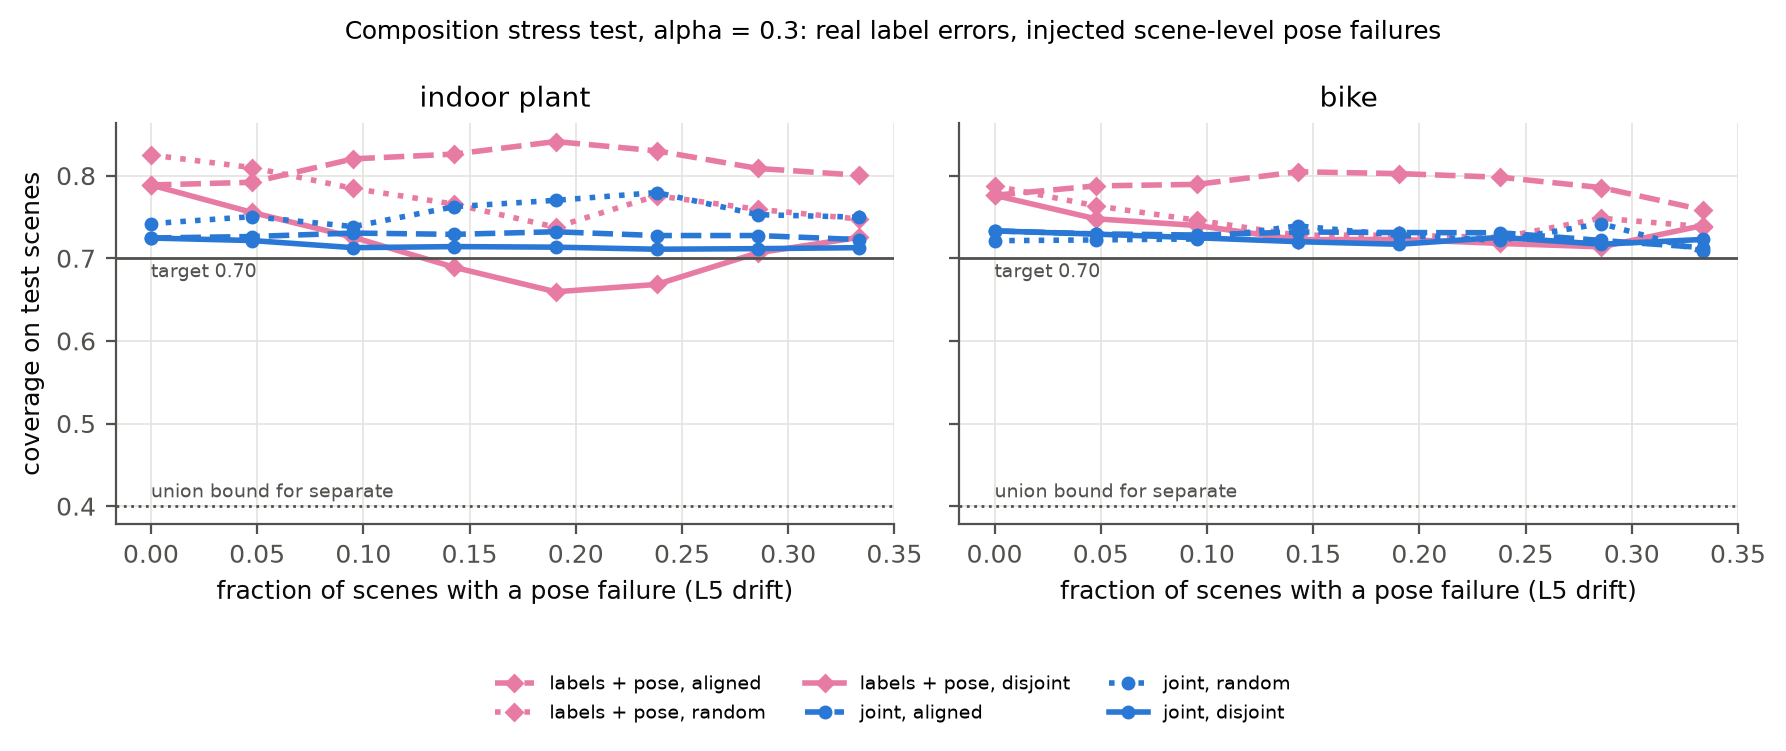
\includegraphics[width=\linewidth]{composition_stress_a03_L5.png}
\caption{Coverage of separate (pink) and joint (blue) margins vs.\ the fraction of scenes with a localization
failure placed where labels are worst (dashed), best (solid) or at random (dotted); $1 - \alpha = 0.7$.}
\label{fig:composition}
\end{figure}

On synthetic drift, which is independent of detector errors, the sum of margins only over-pays
(Table~\ref{tab:coverage}). To probe Proposition~\ref{prop:sep} we keep the real label errors and replace drift by a
scene-level mixture: in $k$ of 21 scenes a localization failure occurs (realizations from L5), in the others drift is
negligible (L1). Failures are placed in the scenes with the worst labels, the best labels, or at random. We use
$\alpha = 0.3$, because at $\alpha = 0.1$ with 13 scenes any failure enters the maximum. The sum covers 0.76--0.84 when
failures coincide with bad labels but only 0.66 at a 0.70 target when they hit scenes with good labels (plant, 19--24\,\%
failing scenes). The joint margin stays at 0.71--0.78 however the failures are placed (Fig.~\ref{fig:composition}).

\subsection{Real odometry and other scenes}

Frame-to-frame odometry without loop closure errs in jumps, mostly during in-place turns near walls: its ATE ranges from
3.5~cm to 3.9~m across scenes, with a median of 78~cm. The labels-only margin then silently covers only 0.67 (bike)
and 0.74 (plant). The joint margin stays valid (0.93, 0.96) but abstains in 60 and 86\,\% of the splits. In missions the
uncalibrated planner finds a path in 23\,\% of the tasks, and 44\,\% of those paths are unsafe; the joint arm abstains in
89\,\% of the tasks. With this pose quality there is no useful certificate, and the method reports it instead of issuing
a false one. Margins calibrated on ReplicaCAD and tested on HM3D scenes~\cite{hm3d} of OSMa-Bench do not transfer: of the
two scenes in which a plant is visible from the trajectory, the detector finds one (miss 0.18~m) and misses the other
(2.9~m), so the guarantee has to be recalibrated where the robot operates.

\section{Discussion and Limitations}

The joint margin is not better than label sets where their assumptions hold. It is better where they fail: under
pose drift and with an open vocabulary. Two of our expectations were wrong. Positive correlation between the errors
makes the sum of margins more conservative; under-coverage appears when rare failures of the two modules hit different
scenes. And with 13 calibration scenes the worst scene sets the margin, so neither a bolder risk level nor better masks
help much. Two attempts to shrink the margin failed: changing the region shape (convex hull, morphological closing) did
not change the miss distance, and a margin scaled by the confidence of each detected fragment did not shrink the
keep-out zone. The bottleneck is confident misses and class swaps of whole objects. If they occur in more than an
$\alpha$ fraction of scenes, no class margin can certify that class, and map metrics such as mIoU do not show it; a
``fraction of scenes with a whole-object miss'' metric would fit mapping benchmarks.

Limitations: one family of 21 simulated scenes and one lighting condition; a box detector rather than a full mapper;
synthetic drift, with real odometry tested only without loop closure; a guarantee that is marginal over scenes and holds
in the planner frame at query time, not during execution; an out-of-distribution check on two scenes. Plant and bike
were chosen as mission classes after seeing that the TV stand abstains; the three-class results are in the code
repository.

\section{Conclusion}

The miss distance in the planner frame is one calibrated quantity that gives a planner a distribution-free guarantee
against label and pose errors together. Margins calibrated on either error alone lose coverage under the other, and the
sum of separate margins depends on an error dependence that is unknown in practice. The remaining price is set by the
worst perception errors, which points to more calibration scenes, SLAM with loop closures and full open-vocabulary
mappers as next steps.

\begin{thebibliography}{99}
\footnotesize
\bibitem{conceptgraphs} Q.~Gu \emph{et al.}, ``ConceptGraphs: Open-vocabulary 3D scene graphs for perception and planning,'' in \emph{Proc. IEEE ICRA}, 2024, pp. 5021--5028, doi: 10.1109/ICRA57147.2024.10610243.
\bibitem{osmabench} M.~Popov \emph{et al.}, ``OSMa-Bench: Evaluating open semantic mapping under varying lighting conditions,'' in \emph{Proc. IEEE/RSJ IROS}, 2025, pp. 10786--10791, doi: 10.1109/IROS60139.2025.11247603.
\bibitem{survey3dsg} D.~Rotondi \emph{et al.}, ``3D scene graphs: Open challenges and future directions,'' arXiv:2606.19383, 2026.
\bibitem{gentle} A.~N.~Angelopoulos and S.~Bates, ``A gentle introduction to conformal prediction and distribution-free uncertainty quantification,'' arXiv:2107.07511, 2021.
\bibitem{sundarsingh} D.~S.~Sundarsingh \emph{et al.}, ``Safe planning in unknown environments using conformalized semantic maps,'' \emph{IEEE Robot. Autom. Lett.}, vol. 11, no. 4, pp. 4921--4928, 2026, doi: 10.1109/LRA.2026.3668466.
\bibitem{pwc} Z.~Mei \emph{et al.}, ``Perceive with confidence: Statistical safety assurances for navigation with learning-based perception,'' \emph{Int. J. Robot. Res.}, vol. 45, no. 6, pp. 938--967, 2025, doi: 10.1177/02783649251378151.
\bibitem{baral} R.~Baral, ``Marginal calibration does not compose: Hidden dependence in modular robot navigation,'' arXiv:2609.23731, 2026 (IROS 2026 workshop).
\bibitem{osmabenchpp} R.~Kurkova, M.~Popov, and S.~Kolyubin, ``OSMa-Bench++: Toward open-ended benchmarking of semantic mapping for manipulation with prompt-generated synthetic scenes,'' arXiv:2605.26831, 2026 (ICRA 2026 workshop).
\bibitem{overconf} J.~M.~Correia Marques, A.~Zhai, S.~Wang, and K.~Hauser, ``On the overconfidence problem in semantic 3D mapping,'' in \emph{Proc. IEEE ICRA}, 2024, pp. 11095--11102, doi: 10.1109/ICRA57147.2024.10611306.
\bibitem{lindemann} L.~Lindemann \emph{et al.}, ``Safe planning in dynamic environments using conformal prediction,'' \emph{IEEE Robot. Autom. Lett.}, vol. 8, no. 8, pp. 5116--5123, 2023, doi: 10.1109/LRA.2023.3292071.
\bibitem{shin2026} J.~Shin, Y.~Ra, and I.~Yang, ``From prediction uncertainty to conformalized distance fields for safe motion planning,'' arXiv:2607.00776, 2026.
\bibitem{learnablecp} D.~Kumar \emph{et al.}, ``Learnable conformal prediction with context-aware nonconformity functions for robotic planning and perception,'' in \emph{Proc. IEEE ICRA}, 2026, arXiv:2509.21955.
\bibitem{tightening} S.~Natraj, B.~Sinopoli, and Y.~Kantaros, ``Conformal constraint tightening for chance-constrained motion planning with unknown dynamics,'' arXiv:2607.22409, 2026.
\bibitem{calafiore2026} G.~C.~Calafiore, ``Bridging conformal prediction and scenario optimization: Discarded constraints and modular risk allocation,'' arXiv:2603.19396, 2026.
\bibitem{pposemem} H.~Sier \emph{et al.}, ``P-POSEMEM: Projective semantic memory for consistent language grounding under pose-graph rewrites,'' arXiv:2609.15475, 2026.
\bibitem{habitat2} A.~Szot \emph{et al.}, ``Habitat 2.0: Training home assistants to rearrange their habitat,'' in \emph{Proc. NeurIPS}, 2021, arXiv:2106.14405.
\bibitem{yoloworld} T.~Cheng \emph{et al.}, ``YOLO-World: Real-time open-vocabulary object detection,'' in \emph{Proc. IEEE/CVF CVPR}, 2024, pp. 16901--16911, doi: 10.1109/CVPR52733.2024.01599.
\bibitem{open3d} Q.-Y.~Zhou, J.~Park, and V.~Koltun, ``Open3D: A modern library for 3D data processing,'' arXiv:1801.09847, 2018.
\bibitem{steinbrucker} F.~Steinbr\"ucker, J.~Sturm, and D.~Cremers, ``Real-time visual odometry from dense RGB-D images,'' in \emph{Proc. IEEE ICCV Workshops}, 2011, pp. 719--722, doi: 10.1109/ICCVW.2011.6130321.
\bibitem{mobilesam} C.~Zhang \emph{et al.}, ``Faster segment anything: Towards lightweight SAM for mobile applications,'' arXiv:2306.14289, 2023.
\bibitem{hm3d} S.~K.~Ramakrishnan \emph{et al.}, ``Habitat-Matterport 3D dataset (HM3D): 1000 large-scale 3D environments for embodied AI,'' in \emph{NeurIPS Datasets and Benchmarks}, 2021, arXiv:2109.08238.
\end{thebibliography}

\end{document}
